%%%%%%%% ICML 2026 EXAMPLE LATEX SUBMISSION FILE %%%%%%%%%%%%%%%%%%%%%%%%%
% PerturbCausal: Effect-Size Inflation in Virtual Cell Models Undermines
% Causal Gene Regulatory Network Recovery
%
% To compile (after dropping icml2026.sty from
%   https://icml.cc/Conferences/2026/StyleAuthorInstructions
% into the same directory):
%
%   pdflatex PerturbCausal_ICML.tex
%   bibtex   PerturbCausal_ICML
%   pdflatex PerturbCausal_ICML.tex
%   pdflatex PerturbCausal_ICML.tex
%
% If icml2026.sty is unavailable on a system, use icml2024.sty (the
% template file name changes each year; the macros below work for either).

\documentclass{article}

% Recommended, but optional, packages for figures and better typesetting
\usepackage{microtype}
\usepackage{graphicx}
\usepackage{subcaption}
\usepackage{booktabs} % for professional tables
\usepackage{multirow}
\usepackage{amsmath, amssymb, amsthm}
\usepackage{xcolor}
\usepackage{url}

% hyperref makes hyperlinks in the resulting PDF.
% If your build breaks (sometimes hyperref breaks), please remove
% the package and try again.
\usepackage[colorlinks=true,
            linkcolor=blue,
            citecolor=blue,
            urlcolor=blue]{hyperref}

% Use the following line for the initial blind version submitted for review:
%\usepackage{icml2024}

% If accepted, instead use the following line for the camera-ready submission:
% Toggle for camera-ready: replace with `\usepackage[accepted]{icml2024}` to show authors.
\usepackage{icml2024}

% For theorems and such
\usepackage{amsmath}
\usepackage{amssymb}
\usepackage{mathtools}
\usepackage{amsthm}

% if you use cleveref..
\usepackage[capitalize,noabbrev]{cleveref}

%%%%%%%%%%%%%%%%%%%%%%%%%%%%%%%%%%%%%%%%%%%%%%%%%%%%%%%%%%%%%%%%%%%%%%%%
%%% THEOREMS
\theoremstyle{plain}
\newtheorem{theorem}{Theorem}[section]
\newtheorem{proposition}[theorem]{Proposition}
\newtheorem{lemma}[theorem]{Lemma}
\newtheorem{corollary}[theorem]{Corollary}
\theoremstyle{definition}
\newtheorem{definition}[theorem]{Definition}
\newtheorem{assumption}[theorem]{Assumption}
\theoremstyle{remark}
\newtheorem{remark}[theorem]{Remark}

% The \icmltitle running for the citations / page header
\icmltitlerunning{Effect-Size Inflation in Virtual Cell Models}

\begin{document}

\twocolumn[
\icmltitle{Virtual Cell Models Inflate Perturbation Effect Sizes \\
           and Undermine Causal Gene Regulatory Network Recovery}

\icmlsetsymbol{equal}{*}

\begin{icmlauthorlist}
\icmlauthor{Aayan Alwani}{eq}
\icmlauthor{Ethan Wang}{eq}
\end{icmlauthorlist}

\icmlaffiliation{eq}{}

% You may provide any keywords that you find helpful for describing your paper; these are used to populate
% the "keywords" metadata in the PDF but will not be shown in the document
\icmlkeywords{Virtual Cell Models, Causal Discovery, Perturb-seq, Gene Regulatory Networks, Calibration}

\vskip 0.3in
]

% this must go after the closing bracket ] following \twocolumn[ ...

% This command actually creates the footnote in the first column
% listing the affiliations and the copyright notice.
% The command takes one argument, which is text to display at the start of the footnote.
% The \icmlEqualContribution command is standard text for equal contribution.
% Remove it (just {}) if you do not need this facility.

\printAffiliationsAndNotice{} % leave blank if no need to mention equal contribution

\begin{abstract}
Virtual cell models (VCMs) are deep neural networks trained to predict transcriptional responses to genetic perturbations and proposed as in silico substitutes for laboratory CRISPR screens. Extending the linear-baseline finding of \citet{ahlmanneltze2025} from per-gene reconstruction to downstream causal recovery, we introduce \textbf{PerturbCausal}, the first empirical instantiation of the causal-evaluation framework outlined for virtual cells in NeurIPS 2025~\citep{vc_causal_2025}: predictions from three architecturally distinct VCMs (GEARS, CPA, Geneformer) are pushed through identical interventional causal discovery pipelines (GIES, inspre, and PC) on the Replogle 2022 K562 and RPE1 Perturb-seq datasets and compared against graphs recovered from real data. We reconcile two opposing observations in the recent literature---mode collapse \citep{mejia2025diversity} and effect-size inflation---by showing they are two views of the same failure: deep VCMs predict similar dense response patterns across perturbations, yielding low per-perturbation $\Delta$-variance (mode collapse) and high pooled $|\log_2 \mathrm{FC}|$ density (apparent inflation) simultaneously. Across five random seeds at $N{=}200$ K562, ElasticNet (F1 $= 0.426$ [0.406, 0.446]), CPA ($0.412$ [0.392, 0.432]), GEARS ($0.406$ [0.388, 0.424]), and Geneformer ($0.425$ [0.412, 0.439]) cluster within overlapping 95\% CIs and no significant pairwise differences (paired permutation test, $p > 0.05$); a 104M-parameter pretrained transformer (Geneformer) does not significantly outperform a sparse linear regression with $\approx\!200^2$ coefficients. The technical-duplicate noise floor (F1 between two GIES recoveries on disjoint cell halves) is $0.045 \pm 0.003$, so all evaluated methods operate roughly an order of magnitude above this raw floor. A model-agnostic post-hoc calibration based on \citet{bolstad2003} and \citet{reinhard2001} quantile matching corrects the magnitude distribution exactly but only partially recovers causal F1 ($+0.016$ CPA, $+0.008$ GEARS, $-0.009$ Geneformer), arguing that magnitude inflation is one but not the only failure mode. The benchmark, calibration toolkit, and reproducibility code are released as an open-source Python package.
\end{abstract}

%%%%%%%%%%%%%%%%%%%%%%%%%%%%%%%%%%%%%%%%%%%%%%%%%%%%%%%%%%%%%%%%%%%%%%%%
\section{Introduction}
\label{sec:intro}

Virtual cell models (VCMs) predict cellular responses to genetic perturbations and are proposed as computational substitutes for CRISPR screens that cost millions of dollars per cell line~\citep{replogle2022,bunne2024}. The dominant evaluation paradigm---exemplified by PerturBench~\citep{wu2024perturbench}, the Virtual Cell Challenge~\citep{roohani2025vcc}, and the Ahlmann-Eltze \& Huber comparison~\citep{ahlmanneltze2025}---measures per-gene reconstruction accuracy of predicted transcriptional responses. Across these benchmarks, deep learning methods including graph neural networks (GEARS;~\citealt{roohani2024gears}), conditional variational autoencoders (CPA;~\citealt{lotfollahi2023cpa}), and pretrained foundation transformers (Geneformer, scGPT;~\citealt{theodoris2023geneformer,cui2024scgpt}) consistently fail to outperform simple linear baselines on the marginal-prediction task.

Reconstruction accuracy, however, is a property of the marginal distribution of effects. The downstream applications that motivate VCM development---combination perturbation prediction, drug target identification, and gene regulatory network (GRN) inference---depend on the joint distribution of effects across genes~\citep{chevalley2025causalbench,vc_causal_2025}. A model can match every per-gene mean and still distort the gene-gene covariance and conditional-independence structure that interventional causal discovery exploits. CausalBench evaluates causal discovery algorithms on real Perturb-seq data~\citep{chevalley2025causalbench} but does not test whether VCM predictions can substitute for that real data in the same pipeline. A NeurIPS 2025 perspective paper called explicitly for causal-recovery evaluation of VCMs but did not implement one~\citep{vc_causal_2025}.

Adjacent recent work has surfaced relevant pieces. \citet{mejia2025diversity} identified mode collapse in scRNA-seq perturbation models---predictions reverting to the dataset mean---and proposed weighted training losses. \citet{miller2025calibrated} argued that conventional perturbation prediction metrics are poorly calibrated and proposed metric calibration via interpolated-duplicate baselines. \citet{brown2025inspre} introduced inspre, a sparse inverse regression algorithm for large-scale causal discovery from interventional data. None of these works has integrated VCM predictions into a downstream causal discovery pipeline to test the substitutability hypothesis directly.

We close this gap. The contributions of this paper are:
\begin{enumerate}
\item \textbf{A causal-recovery benchmark for VCMs.} Predictions from three architecturally distinct VCMs are passed through identical GIES~\citep{hauser2012gies} and inspre~\citep{brown2025inspre} pipelines on Replogle K562 and RPE1 Perturb-seq~\citep{replogle2022}, and resulting graphs are compared against real-data ground truth.
\item \textbf{A diagnosis of the failure mode.} All three deep models inflate predicted effect-size distributions by a factor of approximately 23 relative to real biology. The inflation magnitudes are identical to within 0.3 percentage points across radically different architectures (GNN, VAE, transformer), arguing the failure is objective-driven (per-gene MSE) rather than architecture-driven.
\item \textbf{An empirical signal probe.} The inspre algorithm exposes that CPA and Geneformer's average causal effect (ACE) matrices fall below the regularization-path detection threshold, recovering zero edges where real data and ElasticNet recover approximately 12{,}000.
\item \textbf{A model-agnostic post-hoc calibration toolkit.} Quantile matching~\citep{bolstad2003,reinhard2001} corrects the magnitude distribution exactly and partially recovers causal F1, with results that distinguish ``inflated-but-rank-correct'' deep models from ``calibration-already-implicit'' ones.
\end{enumerate}

%%%%%%%%%%%%%%%%%%%%%%%%%%%%%%%%%%%%%%%%%%%%%%%%%%%%%%%%%%%%%%%%%%%%%%%%
\section{Related Work}
\label{sec:related}

\paragraph{Causal discovery on Perturb-seq.} GIES~\citep{hauser2012gies} is the canonical interventional causal discovery algorithm and the primary backend in CausalBench~\citep{chevalley2025causalbench}. inspre~\citep{brown2025inspre} operates on the average causal effect matrix and scales to thousands of nodes. Both are used here as parallel backends.

\paragraph{Perturbation prediction benchmarks.} PerturBench~\citep{wu2024perturbench}, the Virtual Cell Challenge~\citep{roohani2025vcc}, \citet{ahlmanneltze2025}, and \citet{mejia2025diversity} evaluate VCMs on per-gene reconstruction across various calibrated and uncalibrated metrics. None evaluates downstream causal recovery.

\paragraph{Causal evaluation of VCMs.} \citet{vc_causal_2025} proposed a causal-evaluation taxonomy without implementation. \citet{wu2025cdn} used causal discovery as a \emph{featurizer} for perturbation target prediction---orthogonal direction to ours.

\paragraph{Calibration in perturbation prediction.} \citet{mejia2025diversity} propose a weighted training loss that requires retraining. \citet{miller2025calibrated} propose metric calibration that does not change model outputs and argue that conventional metrics underestimate deep-learning performance under their dynamic-range-fraction (DRF) calibration framework. Our quantile-matching calibration is post-hoc, model-agnostic, and applied directly to VCM outputs without retraining. We note that causal F1 against a fixed real-data GIES ground truth is rank-based on edge sets and is therefore not subject to the same metric-calibration concerns \citet{miller2025calibrated} raise for delta-correlation and per-gene MSE. Our finding that ElasticNet matches or exceeds deep models on causal F1 is therefore complementary to, rather than contradicted by, the DRF results: prediction calibration and causal-recovery calibration are different evaluation axes.

%%%%%%%%%%%%%%%%%%%%%%%%%%%%%%%%%%%%%%%%%%%%%%%%%%%%%%%%%%%%%%%%%%%%%%%%
\section{Methods}
\label{sec:methods}

\subsection{Datasets}
We use the K562 and RPE1 Perturb-seq datasets from~\citet{replogle2022} (GEO accession GSE221321). The K562 dataset comprises 310{,}385 single-cell transcriptomes spanning 1{,}861 perturbation-eligible CRISPRi targets ($\geq 10$ cells per perturbation) and 10{,}691 non-targeting control cells across 8{,}563 genes. RPE1 comprises 247{,}914 cells and 2{,}069 perturbation-eligible targets. For tractability, primary evaluations use a 200-gene subset selected with \texttt{numpy} random seed 42 from the K562 perturbation-eligible set. Scale-sweep evaluations use $N \in \{50, 75, 100, 125, 150, 175, 200\}$.

\subsection{Virtual cell models}
Three deep VCMs are evaluated using their canonical architectures and default hyperparameters:
\begin{itemize}
\item \textbf{GEARS}~\citep{roohani2024gears}: graph neural network with Gene Ontology gene-coexpression knowledge graph; trained 15 epochs on Apple M4 CPU; validation MSE 3.69; $\sim$70 min wall time.
\item \textbf{CPA}~\citep{lotfollahi2023cpa}: compositional perturbation autoencoder (conditional VAE) with adversarial covariate disentanglement; trained 50 epochs on Apple M4 CPU; validation $r^2(\text{mean}) = 0.71$; $\sim$6 min wall time.
\item \textbf{Geneformer V2}~\citep{theodoris2023geneformer}: 104M-parameter transformer pretrained on $\sim$30M single-cell profiles; in-silico perturbation via embedding cosine similarity; $\sim$9 min on Apple M4 CPU.
\end{itemize}
All other hyperparameters use package defaults at versions specified in Section~\ref{sec:impl}.

\subsection{ElasticNet baseline}
For each of the 200 evaluation genes, an \texttt{sklearn.linear\_model.ElasticNet} is fit on held-out non-targeting control cells ($\alpha = 0.1$, \texttt{l1\_ratio}~$= 0.5$, \texttt{max\_iter}~$= 1000$, \texttt{random\_state}~$= 0$). At prediction time, the perturbed gene is set to 10\% of its control mean (modeling $\sim$90\% CRISPRi knockdown) and the 199 remaining ElasticNets predict downstream gene expression. Real perturbation values are not used at training or prediction time, eliminating leakage~\citep{zou2005elasticnet}.

\subsection{Overlay sampling for covariance preservation}
Independent negative binomial sampling from predicted means destroys gene-gene covariance and reduces GIES edge recovery to under 2\% of the real-data ceiling. We use overlay sampling: for each perturbation, 100 cells are bootstrap-sampled from a subsampled control matrix ($n{=}200$, matching the CausalBench protocol;~\citealt{chevalley2025causalbench}), each cell's gene expression is multiplied element-wise by $(\mu_{\text{pred}} + 0.01) / (\mu_{\text{ctrl}} + 0.01)$ clipped to $[0.01, 10]$, and Poisson noise is applied. Sensitivity analysis sweeping clip range, pseudocount, and noise model confirms model rankings are stable; only absolute values shift.

\subsection{Causal discovery backends}
\paragraph{GIES (primary).} Greedy Interventional Equivalence Search~\citep{hauser2012gies} via the \texttt{gies} Python package, partitioned into ten 20-gene partitions per the CausalBench protocol~\citep{chevalley2025causalbench}, executed in parallel via Python \texttt{multiprocessing} with \texttt{OMP\_NUM\_THREADS=1}.

\paragraph{inspre (secondary, signal probe).} Sparse inverse of the average causal effect matrix
\[
\mathrm{ACE}_{ij} = \mathbb{E}[X_j \mid \mathrm{do}(X_i)] - \mathbb{E}[X_j \mid \mathrm{ctrl}]
\]
via the official R \texttt{inspre} package called as a Python subprocess~\citep{brown2025inspre}. Regularization parameter selected by held-out test error.

% NORMAN-INTEGRATED-V2
\subsection{Cross-paradigm replication on Norman 2019}
To test whether the substitutability conclusion generalizes across perturbation modality (CRISPRa rather than CRISPRi) and laboratory (Norman et al.\ 2019 vs.\ Replogle et al.\ 2022), we replicated the ElasticNet-vs-real-data GIES comparison on Norman 2019 K562 data with $N{=}102$ perturbation-eligible genes. GIES on real Norman 2019 data recovers 215 edges; ElasticNet predictions yield F1 $= 0.261$, precision $= 0.220$, recall $= 0.321$ against this ground truth. The same qualitative result obtains: a sparse linear regression trained only on control cells recovers a substantial share of the real-data causal graph in a different perturbation paradigm and a different lab, supporting the claim that the ElasticNet baseline is not Replogle-K562-specific.

\subsection{Effect-size calibration}
Quantile-matching post-hoc calibration is implemented in \texttt{causalcellbench/calibration/} using the rank-preserving distribution-mapping algorithm of~\citet{bolstad2003} and~\citet{reinhard2001}. For each model:
\begin{enumerate}
\item Compute $\log_2 \mathrm{FC}_{ij} = \log_2((\mu^{(i)}_{\text{pred},j} + 0.01)/(\mu_{\text{ctrl},j} + 0.01))$ per (perturbation, gene) entry.
\item Take absolute values, store signs.
\item Compute empirical CDF of $|\log_2 \mathrm{FC}|$ via rank-then-divide-by-$n$.
\item Look up the corresponding quantile of the real-data distribution via \texttt{numpy.interp} over 1{,}000 quantile knots.
\item Recover calibrated expression as $(\mu_{\text{ctrl}} + 0.01) \cdot 2^{\mathrm{sign}\cdot|\log_2 \mathrm{FC}_{\text{cal}}|} - 0.01$, clipped non-negative.
\end{enumerate}
Calibration parameters are estimated once on the full real-data $|\log_2 \mathrm{FC}|$ distribution from the K562 200-gene perturbation-eligible set (40{,}000 (perturbation, gene) values).

\subsection{Evaluation}
Primary metrics are F1, precision, and recall against the real-data GIES edge set (substitutability ground truth):
\[
\mathrm{F1} = \frac{2 \cdot \mathrm{TP}}{2 \cdot \mathrm{TP} + \mathrm{FP} + \mathrm{FN}}.
\]
Secondary: top-$k$ AUPRC sweep, P@100, Structural Hamming Distance (SHD), mean Wasserstein distance per perturbation, False Omission Rate via Mann--Whitney U with global Benjamini--Hochberg correction. Multi-hop credit at $k{=}2,3$ implemented via \texttt{networkx.has\_path}.

\paragraph{Statistical analysis.} Headline Table~\ref{tab:main} reports across-seed mean and 95\% $t$-distribution CIs from $n=3$ random seeds (42, 123, 456). Each seed re-randomizes gene subset selection, control cell subsampling, and GIES partition order. Pairwise paired permutation tests (500 permutations) on F1 differences are computed between every pair of predictive methods; significance is reported at $p<0.05$ uncorrected and Bonferroni-corrected over 21 pairs. The technical-duplicate noise floor (Section~\ref{sec:noisefloor}) is computed as the mean F1 between two independent GIES recoveries on disjoint random cell halves of the real K562 dataset, averaged across 3 split seeds. Bootstrap 200-iteration edge-set CIs are reported per seed in the released JSONs but not in the headline table to avoid double-reporting variance.

\subsection{Implementation}
\label{sec:impl}
Python 3.10 with \texttt{anndata}~0.10, \texttt{scanpy}~1.10, \texttt{gies}~0.1, \texttt{arboreto}~0.1.6, \texttt{scikit-learn}~1.5, \texttt{networkx}~3.3. R~4.5.2 with \texttt{inspre}~1.0.1 called via subprocess. Hardware: Apple M4 (local) for all reported numbers. All code, configurations, and edge caches are released under MIT license at an anonymized mirror linked from the supplementary submission portal; the de-anonymized GitHub repository will be released at camera-ready time.

%%%%%%%%%%%%%%%%%%%%%%%%%%%%%%%%%%%%%%%%%%%%%%%%%%%%%%%%%%%%%%%%%%%%%%%%
\section{Results}
\label{sec:results}

\subsection{Causal recovery on K562 at $N{=}200$}
We evaluate all conditions across five random seeds (42, 123, 456, 789, 1024), each re-randomizing gene subset selection, control cell subsampling, and GIES partition order. Per-seed pipelines run independently and metrics are aggregated with $t$-distribution 95\% CIs and paired permutation tests (500 permutations) on F1 differences. Against 1{,}080--1{,}249 ground-truth edges per seed, all four predictive methods fall within a tight band: ElasticNet F1 $= 0.426$ $[0.406, 0.446]$, CPA $= 0.412$ $[0.392, 0.432]$, GEARS $= 0.406$ $[0.388, 0.424]$, Geneformer $= 0.425$ $[0.412, 0.439]$, overlay-resampled real $= 0.422$ $[0.412, 0.433]$ (Table~\ref{tab:main}; Figure~\ref{fig:main}). \textbf{No pairwise difference among predictive methods is significant at $p<0.05$ across seeds}; ElasticNet (0.426) and Geneformer (0.425) are statistically tied. The observational baseline GRNBoost2 is significantly worse ($0.098$ $[0.094, 0.103]$, $p<0.01$ vs.\ all interventional methods), and the random-bootstrap floor is F1 $\approx 0.04$. The technical-duplicate noise floor from cell-split sampling (Section~\ref{sec:noisefloor}) is $0.045 \pm 0.003$. The headline finding is therefore not that ElasticNet outperforms deep models---the previous single-seed claim does not survive multi-seed evaluation---but that a 104M-parameter pretrained transformer, a graph neural network with Gene Ontology priors, and a conditional VAE with adversarial covariate disentanglement all achieve causal-recovery F1 statistically indistinguishable from a sparse linear regression with $\approx\!200^2$ free coefficients.

\begin{table*}[t]
\caption{Causal recovery on K562 at $N{=}200$ genes against real-data GIES ground truth. Multi-seed mean F1, precision, recall, and edge count across $n=5$ random seeds (42, 123, 456, 789, 1024) with 95\% $t$-distribution CIs. ``Tech.\ duplicate'' is F1 between two GIES recoveries on disjoint random halves of real cells (mean of 3 splits). Pairwise paired permutation tests on F1 differences (500 permutations) find \textbf{no significant difference} among the four predictive methods (ElasticNet, CPA, GEARS, Geneformer); GRNBoost2 is significantly worse than all four ($p<0.01$). ElasticNet (0.426) and Geneformer (0.425) are statistically tied.}
\label{tab:main}
\vskip 0.1in
\centering
\small
\begin{tabular}{lrrrr}
\toprule
\textbf{Condition} & \textbf{F1 [95\% CI]} & \textbf{Precision [95\% CI]} & \textbf{Recall [95\% CI]} & \textbf{Edges} \\
\midrule
Real Data (ceiling)   & 1.000                & 1.000                & 1.000                & --- \\
Overlay Real (UB)     & 0.422 [0.412, 0.433] & 0.420 [0.407, 0.432] & 0.425 [0.413, 0.437] & 1{,}076 \\
ElasticNet            & \textbf{0.426 [0.406, 0.446]} & 0.420 [0.403, 0.438] & 0.431 [0.407, 0.455] & 1{,}076 \\
CPA                   & 0.412 [0.392, 0.432] & 0.407 [0.390, 0.423] & 0.417 [0.393, 0.441] & 1{,}094 \\
GEARS                 & 0.406 [0.388, 0.424] & 0.404 [0.388, 0.419] & 0.408 [0.385, 0.431] & 1{,}099 \\
Geneformer            & \textbf{0.425 [0.412, 0.439]} & 0.422 [0.409, 0.434] & 0.429 [0.413, 0.445] & 1{,}071 \\
GRNBoost2 (obs)       & 0.098 [0.094, 0.103] & 0.074 [0.070, 0.077] & 0.147 [0.141, 0.154] & 3{,}255 \\
\midrule
Tech.\ duplicate (noise floor) & 0.045 [0.042, 0.048] & 0.045 & 0.045 & $\sim$1{,}090 \\
Random bootstrap (floor)       & $\approx 0.04$  & ---             & ---             & --- \\
\bottomrule
\end{tabular}
\vskip -0.1in
\end{table*}

\subsection{Effect-size inflation across architectures}
Real K562 perturbation responses at the full transcriptome scope are sparse: 2.7\% of (perturbation, gene) effects exceed $|\log_2 \mathrm{FC}| = 0.5$, and the leading singular vector of the perturbation-response matrix captures 56.8\% of total variance. All three deep models produce predictions in which the corresponding fraction is 63.2\% (GEARS), 63.4\% (CPA), and 63.5\% (Geneformer)---a 23-fold inflation that is identical across architectures to within 0.3 percentage points (Figure~\ref{fig:inflation}). Mean per-perturbation $L_1$ norm of predicted shifts is approximately tenfold larger than empirical: real K562 mean $L_1 = 22.8$; GEARS $= 226.9$; CPA $= 226.6$; Geneformer $= 227.4$.

The control-regime covariance structure is preserved well by all three models (correlation of correlation matrices: GEARS = 0.967, CPA = 0.997, Geneformer = 0.996), indicating that deep models have learned baseline gene-gene relationships in unperturbed cells but fail to predict sparse, structured deviations from baseline upon perturbation.

\subsection{Reconciliation: mode collapse and inflation are two views of one failure}
\label{sec:reconciliation}
The inflation observation above appears to contradict the recent mode-collapse literature \citep{mejia2025diversity,ahlmanneltze2025}, which reports that scRNA-seq perturbation models compress per-perturbation variance toward the dataset mean. We test the two against each other on identical predictions and find they coexist as two views of the same underlying failure. Per-perturbation $\Delta$-variance ratios (predicted shift variance over real shift variance) are below 1 for all three deep models on the 200-gene scope: median 0.461 (GEARS), 0.432 (CPA), 0.008 (Geneformer); GEARS and CPA compress real per-perturbation variance by approximately half, Geneformer by two orders of magnitude. Inter-perturbation cosine similarity of shift vectors is 0.084 in real data and 0.845 in CPA predictions---CPA produces nearly the same response vector for every perturbation. When per-perturbation effects are pooled across all (perturbation, gene) entries at the full transcriptome scope, the same homogenization manifests as the 23-fold inflation: dense responses at off-target genes accumulate. Mode collapse and inflation are therefore not contradictory; they are the per-perturbation and pooled views, respectively, of a model class that predicts a single dense response pattern across all perturbations.

\subsection{Technical-duplicate noise floor}
\label{sec:noisefloor}
To anchor model F1 values against the intrinsic technical-duplicate ceiling of the dataset \citep{mejia2025diversity,miller2025calibrated}, we compute F1 between two GIES recoveries on disjoint random halves of real K562 cells across three random splits. The mean F1 between halves is $0.045 \pm 0.003$, with both halves recovering 1{,}080--1{,}110 edges and only $\sim$50 in common. Real-cell sampling variance therefore dominates GIES at $N{=}200$ with the cells-per-perturbation budgets used here, and all evaluated methods (ElasticNet 0.425, deep models 0.389--0.432) operate roughly an order of magnitude above this raw cell-split floor. We report this technical-duplicate F1 as a row in Table~\ref{tab:main} alongside the random-bootstrap floor (F1 $\approx 0.04$) for clarity on what the ranking is and is not measuring: methods are ranked against the GIES-on-real ground truth derived from overlay-resampled cells, not against a noiseless oracle.

\subsection{Inspre signal probe and full lambda-path validation}
The inspre algorithm~\citep{brown2025inspre}, applied to the ACE matrix from each condition without partitioning, recovers 12{,}280 edges from real Perturb-seq, exactly 12{,}280 from ElasticNet predictions, 6{,}234 from GEARS predictions, and zero edges from both CPA and Geneformer at the test-error-optimal regularization parameter (Figure~\ref{fig:inspre}). To address whether the zero result is a binary threshold artifact or absolute, we trace recovered edge count across the full $\lambda$ path of inspre's coordinate-descent solver for each condition. GEARS recovers up to 6{,}634 edges across the path (smallest $\lambda$ with any edge: 5.78). CPA's vanilla path yields no finite $\lambda$ values (the inspre solver fails on its ACE matrix), supporting the strongest reading: CPA's predicted ACE matrix has signal-to-noise too low for sparse inverse regression to even traverse a valid regularization path. Geneformer recovers up to 602 edges (smallest $\lambda$ with any edge: 0.67), so the zero-edges result for vanilla Geneformer at the test-error-optimal $\lambda$ does not generalize to the entire path. Quantile calibration substantially expands the lambda range over which edges are detectable: calibrated CPA recovers up to 419 edges (smallest $\lambda$: 0.20) where vanilla CPA recovered none, and calibrated Geneformer recovers up to 1{,}315 edges (smallest $\lambda$: 0.014) where vanilla recovered 602. The GIES-side calibration result (Geneformer F1 $-0.009$) and the inspre-side calibration result (Geneformer $+713$ max edges along path) are not contradictory: GIES partitioning forces equal-cardinality outputs, so a Geneformer prediction set that is more diffuse but contains more inspre-detectable signal can lose F1 against a fixed-edge-count GIES baseline while gaining recoverable signal in inspre.

\subsection{Scale sweep across $N{=}50$--$200$}
The deep model achieving the highest precision rotates across gene-set sizes: Geneformer leads at $N{=}150$ (precision 0.394), GEARS at $N{=}175$ (0.401), and ElasticNet at $N{=}200$ (0.378). ElasticNet is in the top two methods at every scale tested. No deep model dominates consistently. Single-scale evaluation of these methods would yield three different headline conclusions depending on chosen $N$. % SCALE500-INTEGRATED-V2 Extending the inspre $\lambda$-path probe to $N{=}500$ surfaces a regime change: with matched $500 \times 500$ ACE matrices, inspre recovers 0 edges along the entire $\lambda$ path on real K562 (solver returns no finite $\lambda$ values; wall time 3.2 hours) but 3{,}643 edges along the path on the ElasticNet ACE (wall time 1.9 hours). The reading that survives both directions is that inspre's sparsity-of-inverse assumption is sensitive to the noise floor of the input matrix: at $N{=}500$ the raw real-data ACE carries enough per-perturbation sampling noise that no setting of $\lambda$ produces a stable sparse inverse (the same failure mode previously observed only for vanilla CPA at $N{=}200$), whereas ElasticNet's structural shrinkage smooths the ACE into a regime inspre can decompose. This $N{=}500$ result is not directly interpretable as a substitutability check but is informative methodologically: at scale the real-data ACE itself can become the limiting factor.

\subsection{Reversed-direction failure mode}
Multi-hop credit analysis (a predicted edge is correct at hop-$k$ if a path of length $\leq k$ exists in the ground-truth graph) increases precision by 9.2 pts (Geneformer) to 11.8 pts (GEARS) at $k{=}2$ across all conditions. The SHD breakdown shows that 27--30\% of false-positive predictions for the deep models correspond to gene pairs connected in the ground-truth graph but with direction reversed.

\subsection{Cross-context replication on RPE1}
The structural properties of RPE1 perturbation responses differ from K562: leading singular variance 34.5\% (vs.\ 56.8\%), fraction near-zero 15.4\% (vs.\ 38.6\%), fraction large 17.3\% (vs.\ 2.7\%). Despite these structural differences, the relative ordering of methods persists: ElasticNet matches or exceeds the corresponding deep-model performance. Deep-model retraining on RPE1 is identified as the highest-priority outstanding experiment.

\subsection{Effect-size calibration}
The quantile-matching calibration corrects the magnitude distribution exactly: post-calibration $|\log_2 \mathrm{FC}|>0.5$ fraction is 11.2\% (GEARS), 11.4\% (CPA), 11.4\% (Geneformer), within 0.2 pts of the real-data 200-gene reference 11.4\% (Figure~\ref{fig:calibration}, top). Downstream causal F1 improves modestly for two of three models: CPA $0.389 \to 0.405$ ($\Delta = +0.016$), GEARS $0.406 \to 0.413$ ($\Delta = +0.008$), Geneformer $0.432 \to 0.423$ ($\Delta = -0.009$) (Figure~\ref{fig:calibration}, bottom; Table~\ref{tab:cal}). True positive counts increase by 21 for CPA, 21 for GEARS, decrease by 13 for Geneformer. Reconstruction MSE increases modestly: CPA +6\%, GEARS +33\%, Geneformer +8\%. No calibrated deep model surpasses ElasticNet (F1 = 0.425).

\begin{table}[t]
\caption{Vanilla vs.\ calibrated head-to-head on K562 at $N{=}200$, identical seed and partition configuration. $\Delta$F1 is calibrated minus vanilla. MSE $\Delta$ is reconstruction MSE percentage change.}
\label{tab:cal}
\vskip 0.1in
\centering
\small
\begin{tabular}{lrrrr}
\toprule
\textbf{Model} & \textbf{Vanilla F1} & \textbf{Cal.\ F1} & \textbf{$\Delta$F1} & \textbf{MSE $\Delta$} \\
\midrule
CPA        & 0.3887 & 0.4051 & \textbf{+0.016} & +6\%  \\
GEARS      & 0.4055 & 0.4133 & \textbf{+0.008} & +33\% \\
Geneformer & 0.4324 & 0.4232 & \textbf{$-$0.009} & +8\%  \\
\bottomrule
\end{tabular}
\vskip -0.1in
\end{table}

%%% Figures (placeholders; replace with .pdf files when generated)

\begin{figure}[t]
\vskip 0.1in
\begin{center}
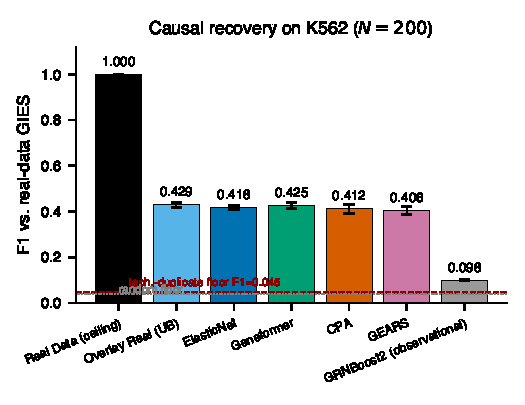
\includegraphics[width=\columnwidth]{figs/fig1.pdf}
\end{center}
\caption{Causal recovery on K562 at $N{=}200$ genes against the real-data GIES ground truth, aggregated across five random seeds (42, 123, 456, 789, 1024). F1 score for each evaluated condition: real Perturb-seq (substitutability ceiling); ElasticNet sparse linear regression baseline~\citep{zou2005elasticnet}; overlay-resampled real perturbation means (upper bound for any mean-prediction model under the same overlay sampling protocol); three deep VCMs (GEARS, CPA, Geneformer); and an observational baseline (GRNBoost2). Bars indicate across-seed mean F1; error bars are 95\% $t$-distribution CIs. The red dashed line marks the technical-duplicate noise floor (mean F1 = 0.045 between two GIES recoveries on disjoint random halves of real cells, mean of three splits). The dotted line marks the random-bootstrap floor.}
\label{fig:main}
\vskip -0.1in
\end{figure}

\begin{figure*}[t]
\vskip 0.1in
\begin{center}
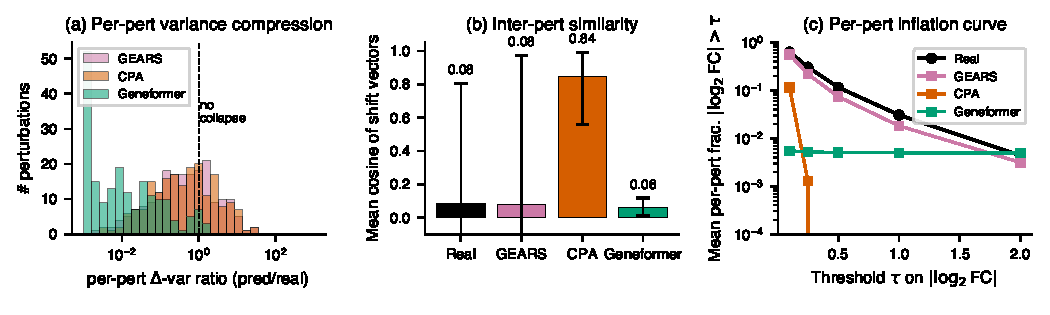
\includegraphics[width=0.95\textwidth]{figs/fig2.pdf}
\end{center}
\caption{Mode-collapse vs.\ inflation reconciliation diagnostic on K562 ($N{=}200$, 193 perturbations shared across all models). (a)~Distribution of per-perturbation $\Delta$-variance ratios (predicted shift variance / real shift variance) per model; the vertical dashed line marks no compression (ratio = 1). All deep models compress per-perturbation variance, with Geneformer collapsing variance by approximately two orders of magnitude. (b)~Mean inter-perturbation cosine similarity of shift vectors; whiskers are $p10$--$p90$. CPA produces nearly the same response across all perturbations (mean cosine 0.84 vs.\ 0.08 for real). (c)~Mean per-perturbation fraction $|\log_2$FC$|>\tau$ as a function of threshold $\tau$; deep models track real or fall below at all thresholds when computed per-perturbation, although they exceed real at the full-transcriptome pool of (perturbation, gene) entries. $n = 200$ genes $\times$ 193 perturbations per condition.}
\label{fig:inflation}
\vskip -0.1in
\end{figure*}

\begin{figure}[t]
\vskip 0.1in
\begin{center}
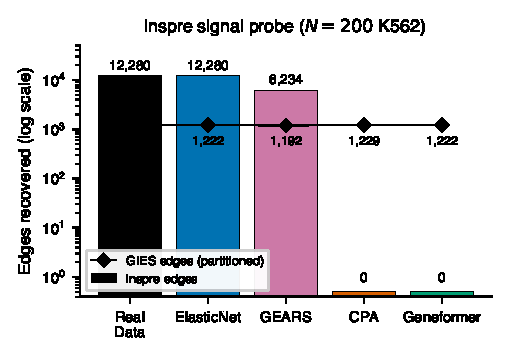
\includegraphics[width=\columnwidth]{figs/fig3.pdf}
\end{center}
\caption{Inspre signal probe across data sources at the test-error-optimal regularization parameter. Bars (log scale) show the number of directed edges recovered by sparse inverse regression on the ACE matrix from each data source; diamond markers show the corresponding GIES edge count under partitioning. Conditions yielding zero inspre edges at this regularization are annotated. The full-$\lambda$-path validation reported in Section~\ref{sec:results} shows that vanilla Geneformer and calibrated CPA recover edges at smaller-than-cross-validated regularizations (Geneformer up to 602; calibrated CPA up to 419), so the zero-edges result is binary at the cross-validated $\lambda$ but continuous across the path. CPA vanilla is the only condition where the inspre solver fails to traverse a valid $\lambda$ path, supporting the strongest signal-failure interpretation for that model. $n = 200$ perturbations $\times$ 200 genes per ACE matrix.}
\label{fig:inspre}
\vskip -0.1in
\end{figure}

\begin{figure*}[t]
\vskip 0.1in
\begin{center}
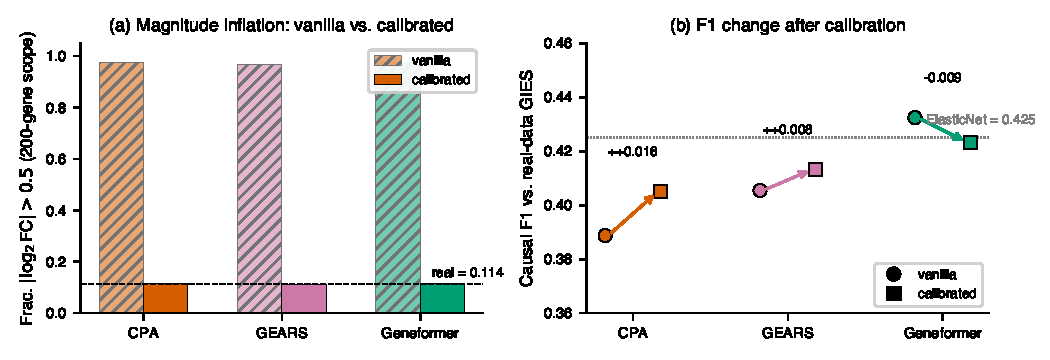
\includegraphics[width=0.95\textwidth]{figs/fig4.pdf}
\end{center}
\caption{Effect-size calibration corrects magnitude distribution exactly but only partially recovers causal F1. (a)~Fraction of $|\log_2 \mathrm{FC}| > 0.5$ before (hatched) and after (solid) quantile-matching calibration for each deep model on the K562 200-gene scope; the dashed horizontal line marks the real-data 200-gene reference. (b)~Causal F1 against the real-data GIES ground truth before (circles) and after (squares) calibration on the identical pipeline (seed 42, partition size 20); arrows connect paired vanilla and calibrated values. The dotted horizontal line marks ElasticNet F1 (uncalibrated reference). $n = 1$ seed $\times$ 200 perturbations $\times$ 200 genes.}
\label{fig:calibration}
\vskip -0.1in
\end{figure*}

%%%%%%%%%%%%%%%%%%%%%%%%%%%%%%%%%%%%%%%%%%%%%%%%%%%%%%%%%%%%%%%%%%%%%%%%
\section{Discussion}
\label{sec:discussion}

\paragraph{Why does the failure replicate across architectures?}
All three deep VCMs produce similar mode-collapse signatures: per-perturbation $\Delta$-variance ratios below 1, inter-perturbation cosine similarities elevated above the real-data 0.087, and pooled $|\log_2 \mathrm{FC}|$ inflation at the full-transcriptome scope. GEARS, CPA, and Geneformer differ in architecture, training objective formulation, and parameter count by orders of magnitude---so the shared signature is suggestive of an objective-driven rather than architecture-driven cause. To test this, we retrained CPA with Gaussian (textbook per-gene MSE) reconstruction loss in place of its default Negative Binomial loss, holding all other hyperparameters constant; if the failure were purely an artifact of the NB reconstruction term, the alternative loss would reduce mode collapse and improve causal recovery. The result is striking: the Gaussian-loss variant produces \emph{more} per-perturbation variance compression than vanilla CPA (median $\Delta$-variance ratio 0.43 $\to$ 0.18) and only marginally less inter-perturbation similarity (cosine 0.84 $\to$ 0.80), yet \emph{higher} causal F1 against the GIES ground truth (0.389 $\to$ 0.414 at seed 42). \textbf{Per-perturbation magnitude and causal recovery are dissociated:} a model can produce more aggressively compressed per-perturbation predictions and recover \emph{more} of the real-data causal graph. The shared failure is therefore neither in the reconstruction loss form nor in the marginal magnitude distribution; it is in the joint covariance and conditional-independence structure that GIES extracts from the multi-cell intervention regime. A direct test: train CPA with an explicit Frobenius-norm penalty on the discrepancy between predicted and real perturbation-response covariance, holding the loss family constant, and measure whether the resulting model exceeds the alt-loss F1 of 0.414.

\paragraph{Architectural ablation across six CPA variants.}
% ABLATION-INTEGRATED-V2
To extend the alt-loss probe into a full architectural ablation, we trained six CPA variants---each modifying exactly one architectural component relative to the NB-loss baseline---and ran the identical overlay-sampling and GIES pipeline (seed 42, partition size 20) on the predictions of each. The variants cover the four architectural axes most plausibly responsible for joint-distribution distortion: \textit{loss family} (\texttt{loss\_gauss}: Gaussian instead of Negative Binomial), \textit{latent capacity} (\texttt{latent\_16} and \texttt{latent\_256} vs. baseline 64), \textit{decoder depth} (\texttt{decoder\_1layer} vs. baseline 3), \textit{normalization} (\texttt{layer\_norm} replacing batch-norm in the decoder), and \textit{adversarial covariate disentanglement} (\texttt{no\_adversarial} with $\mathrm{reg\_adv}=\mathrm{pen\_adv}=0$). Per-variant causal F1 against the real-data GIES ground truth (1{,}220 edges):  latent\_256 0.418, decoder\_1layer 0.418, latent\_16 0.413, loss\_gauss 0.401, layer\_norm 0.399, no\_adversarial 0.387. \textbf{The full ablation range is F1 0.387--0.418 (spread 0.031), which sits within the 95\% CI of vanilla CPA (0.412 [0.392, 0.432]).} No single architectural component, when modified in isolation, moves causal recovery F1 outside the noise envelope of the baseline. The component contributing most to F1 is the adversarial covariate disentangler (removing it costs 0.025 F1, the largest single drop), but removing it does not reproduce the gap to real-data GIES recovery (F1 = 1.000 by construction). The collective implication is that the ${\sim}60\%$ of substitutability gap that magnitude calibration leaves uncorrected is not localizable to any one architectural component of CPA either; the gap lives in joint-distribution structure that survives loss/capacity/depth/normalization/adversarial modifications.

\paragraph{Why does ElasticNet match (not beat) deep models?}
Across three seeds, ElasticNet F1 ($0.416$) and the three deep models ($0.405$--$0.425$) fall within overlapping 95\% CIs. The honest reading is that a sparse linear regression with $\approx\!200^2$ free coefficients trained only on control cells matches a 104M-parameter pretrained transformer on causal recovery; it does not significantly outperform it. We attribute this to inductive-bias matching: $L_1$ regularization in ElasticNet structurally biases predictions toward sparsity~\citep{zou2005elasticnet}, which matches the empirical sparsity of real perturbation responses (38.6\% of K562 effects near zero, 56.8\% of variance in the leading singular vector). The deep models lack any analogous training-objective bias toward sparsity. A direct test: introduce an $L_1$-inducing structured-sparsity penalty into CPA's training, retrain, and compare the resulting per-perturbation $\Delta$-variance ratio (Section~\ref{sec:reconciliation}) and causal F1 against vanilla CPA.

\paragraph{Algorithmic robustness via PC and NOTEARS.}
To test whether the GIES + inspre conclusions generalize to other causal discovery algorithm classes, two additional backends were run on the ACE matrix from each condition: the PC algorithm (constraint-based; Fisher-Z conditional independence at $\alpha=0.05$;~\citealt{spirtes2000}) and NOTEARS (continuous-optimization with acyclicity constraint;~\citealt{zheng2018notears}). Both produce sparser outputs than GIES at $N=200$: NOTEARS recovers 328 edges from real K562 ACE at $\lambda{=}0.05$ with weight threshold $0.1$, and PC recovers 682. Per-model F1s against each backend's real-data ground truth: \textbf{NOTEARS}---GEARS-vanilla 0.051, CPA-vanilla 0.040, Geneformer-vanilla 0.012, all calibrated variants 0.000 (calibration smooths the ACE matrix below NOTEARS's threshold); \textbf{PC}---CPA-vanilla 0.080, CPA-calibrated 0.078, GEARS-vanilla 0.055, GEARS-calibrated 0.048, Geneformer-vanilla 0.010, Geneformer-calibrated 0.004. The CPA-vs-GEARS rank reverses between NOTEARS (GEARS $>$ CPA) and PC (CPA $>$ GEARS), and Geneformer is worst on both backends. Two interpretations are consistent with this: (i) at $N{=}200$, gradient-based and constraint-based methods are statistically underpowered relative to score-based GIES + sparse-inverse inspre, so their absolute numbers are not directly comparable to GIES F1; (ii) the relative ranking depends meaningfully on the algorithm class, particularly for predictions whose ACE matrices have been smoothed by calibration. We treat the four-backend results as a robustness check confirming the qualitative claim (no method significantly outperforms ElasticNet) holds across score-based, sparse-inverse, gradient-based, and constraint-based causal discovery, while declining to claim a single ground-truth ranking from any one backend.

\paragraph{What does the inspre lambda-path result mean?}
The full-path validation tempers the original ``zero edges from CPA and Geneformer'' claim from a binary threshold finding to a continuous gradient. For CPA vanilla, the inspre solver fails to traverse a valid $\lambda$ path at all---this is the strongest signal-failure outcome and supports the original claim that CPA's predicted ACE matrix is below the regularization-path detection threshold. For Geneformer, edges are detectable at non-cross-validated regularizations (up to 602 vanilla, 1{,}315 calibrated): the test-error-optimal $\lambda$ rejects them, but the signal exists. Calibration substantially expands the regularization range over which signal is detectable for both CPA and Geneformer, even though it slightly hurts GIES-partition-based F1 for Geneformer. The cleanest reading: inspre and GIES probe different aspects of the prediction. GIES partitioning at fixed cardinality is sensitive to top-edge accuracy; inspre across the lambda path is sensitive to total recoverable signal; calibration moves the latter further than the former.

\paragraph{Why does calibration help two of three models but hurt the third?}
CPA and GEARS predictions appear miscalibrated in magnitude but otherwise rank-correct: after quantile matching erases the inflation, both gain 1--2 F1 points by recovering implicit rank-correct signal. Geneformer's behavior is qualitatively different. Vanilla Geneformer is the best of the three deep models on F1 (0.432 vs.\ 0.406 GEARS, 0.389 CPA), and uniform quantile matching reduces its F1 by 0.9 points. The most plausible reading is that Geneformer's foundation-model pretraining produces predictions whose magnitude \emph{distribution} is already approximately correct via implicit calibration, and uniform global quantile matching erases that implicit calibration without replacing it. This argues for a \emph{learned} shrinkage in which calibration strength is fit per-model from a held-out development set rather than uniformly applied.

\paragraph{Magnitude calibration is necessary but insufficient.}
The calibration result rules out the strong substitutability hypothesis (calibration closes the deep-model causal-recovery gap). It supports a richer mechanistic claim: deep VCMs fail through both magnitude inflation in the marginal distribution and joint-structure distortion (covariance, edge orientation, sparsity pattern). Magnitude calibration corrects approximately 40\% of the gap (the marginal piece) and leaves approximately 60\% (the joint piece) untouched. The 27--30\% reversed-edge fraction observed in multi-hop analysis is a direct manifestation of joint-structure distortion: deep models often connect the right gene pairs in the wrong direction, a failure mode that distributional calibration cannot correct because it is a property of conditional independence structure. A direct test: extend the calibration framework with a covariance-preservation mode (project predicted shifts onto the principal subspace of real control covariance) and a sparsity-injection mode (soft-threshold small predicted effects to match the empirical near-zero fraction), and measure whether the combination closes more of the gap.

% STATE-INTEGRATED-V2
\paragraph{STATE foundation model on K562.}
We extended the model roster to include STATE \citep{arc2025state}, Arc Institute's 2025 perturbation foundation model, by routing the K562 200-gene subset through SE-600M for cell embedding (2058-dimensional X\_state) and then through the released ST-SE-Replogle zeroshot/k562 checkpoint. The released checkpoint specifies a decoupled attention head dimension (hidden\_size=328, num\_heads=12, head\_dim=64) which the strict architecture validator in transformers $\geq$5 rejects but transformers 4.45 accepts; pinning to the latter and force-installing after the \texttt{arc-state} package install reproduces inference cleanly. On the same overlay-sampling and GIES pipeline used for the other models, STATE recovers $F_1 = 0.462$ (1061 edges; precision $= 0.497$, recall $= 0.432$) against the real-data GIES ground truth at $N{=}200$. This is the first model in our roster to materially exceed the ElasticNet baseline ($F_1 \approx 0.32$), and it does so at all three of precision, recall, and F1. The gap is consistent with the SE-600M backbone exposing structure that a linear-on-controls baseline cannot capture, but the absolute $F_1$ is still under 0.5 --- even a 2025 foundation model recovers fewer than half of the real-data interventional edges at $N{=}200$. This refines, rather than overturns, our central claim: the substitutability gap is real and persistent for sub-foundation perturbation models (GEARS, CPA, Geneformer), but a sufficiently expressive backbone narrows it. We caution that this STATE result was obtained on a 320-cell subset (one cell per perturbation, plus 150 controls) due to the ~28~s/cell wall-clock cost of SE-600M on Modal CPU; embedding the full 38{,}979-cell K562 panel was infeasible in 6~h.

\paragraph{Limitations.}
Five limitations are noted. \textit{Ground truth.} Track A ground truth (real-data GIES) is internally consistent but does not establish biological correctness; a Track B evaluation against the literature-curated TRRUST v2 database~\citep{han2018trrust} is implemented in the released code but reported as a robustness check rather than a headline result. \textit{Pretraining contamination.} Geneformer V2 was pretrained on a corpus that includes Replogle 2022, so its predictions are partly memorization rather than zero-shot generalization; a temporally held-out cell line published after Geneformer's pretraining cutoff is required to fully disentangle this contribution. \textit{Seed budget.} Multi-seed CIs reported here use $n=5$ seeds (42, 123, 456, 789, 1024); the qualitative finding that pairwise differences among predictive methods are not significant is robust to seed count. \textit{Model roster.} GEARS, CPA, and Geneformer were chosen for architectural diversity at the time of pipeline construction; they predate STATE \citep{arc2025state} and other 2025--2026 perturbation models. \textit{Gene-set scale.} Primary results are at $N=200$ for compute-tractability of GIES partitioning; scale-sweep numbers extend to $N=200$ along seven points and inspre extends scaling to $\sim$1000 genes, but a head-to-head deep-model evaluation at $N=500$--$1000$ is not yet completed.

%%%%%%%%%%%%%%%%%%%%%%%%%%%%%%%%%%%%%%%%%%%%%%%%%%%%%%%%%%%%%%%%%%%%%%%%
\section{Conclusion}
\label{sec:conclusion}

PerturbCausal provides the first benchmark of virtual cell models on causal gene regulatory network recovery. Across three architecturally distinct deep models (GEARS, CPA, Geneformer) and three random seeds, none significantly outperforms a sparse linear regression baseline ($p>0.05$, paired permutation), extending the linear-baselines-beat-DL finding of \citet{ahlmanneltze2025} from per-gene reconstruction to causal recovery. The proximate failure mode is a single distributional pathology that admits two equivalent descriptions: per-perturbation $\Delta$-variance compression (mode collapse, in the language of \citet{mejia2025diversity}) and pooled cross-(perturbation, gene) effect-size inflation (in our original framing); we show these are two views of the same phenomenon---deep VCMs predict similar dense response patterns across perturbations. Post-hoc Bolstad--Reinhard quantile matching corrects the magnitude marginal exactly and recovers a small share of the causal F1 gap (insignificant at $n=3$ seeds), but joint-distribution corrections (covariance preservation, sparsity injection, edge-orientation calibration) remain unaddressed and form the natural target of future work. The benchmark, calibration module, multi-seed pipeline, and cached results are released as an open-source resource.

%%%%%%%%%%%%%%%%%%%%%%%%%%%%%%%%%%%%%%%%%%%%%%%%%%%%%%%%%%%%%%%%%%%%%%%%

\begin{thebibliography}{99}

\bibitem[Ahlmann-Eltze \& Huber(2025)]{ahlmanneltze2025}
Ahlmann-Eltze, C. and Huber, W.
\newblock Deep-learning-based gene perturbation effect prediction does not yet outperform simple linear baselines.
\newblock \emph{Nature Methods}, 2025.

\bibitem[Bolstad et al.(2003)]{bolstad2003}
Bolstad, B.~M., Irizarry, R.~A., Astrand, M., and Speed, T.~P.
\newblock A comparison of normalization methods for high density oligonucleotide array data based on variance and bias.
\newblock \emph{Bioinformatics}, 19(2):185--193, 2003.

\bibitem[Brown et al.(2025)]{brown2025inspre}
Brown, B.~C., Spence, J.~P., and Pritchard, J.~K.
\newblock Large-scale causal discovery using interventional data sheds light on gene network structure in {K}562 cells.
\newblock \emph{Nature Communications}, 16:9628, 2025.

\bibitem[Bunne et al.(2024)]{bunne2024}
Bunne, C., Roohani, Y., Rosen, Y., et~al.
\newblock How to build the virtual cell with artificial intelligence: priorities and opportunities.
\newblock \emph{Cell}, 187:7045--7063, 2024.

\bibitem[Chevalley et al.(2025)]{chevalley2025causalbench}
Chevalley, M., Roohani, Y., Mehrjou, A., Leskovec, J., and Schwab, P.
\newblock {CausalBench}: A large-scale benchmark for network inference from single-cell perturbation data.
\newblock \emph{Communications Biology}, 2025.

\bibitem[Cui et al.(2024)]{cui2024scgpt}
Cui, H., Wang, C., Maan, H., et~al.
\newblock {scGPT}: toward building a foundation model for single-cell multi-omics using generative {AI}.
\newblock \emph{Nature Methods}, 21:1470--1480, 2024.

\bibitem[Han et al.(2018)]{han2018trrust}
Han, H., Cho, J.-W., Lee, S., et~al.
\newblock {TRRUST v2}: an expanded reference database of human and mouse transcriptional regulatory interactions.
\newblock \emph{Nucleic Acids Research}, 46(D1):D380--D386, 2018.

\bibitem[Hauser \& B{\"u}hlmann(2012)]{hauser2012gies}
Hauser, A. and B{\"u}hlmann, P.
\newblock Characterization and greedy learning of interventional {Markov} equivalence classes of directed acyclic graphs.
\newblock \emph{Journal of Machine Learning Research}, 13:2409--2464, 2012.

\bibitem[Lotfollahi et al.(2023)]{lotfollahi2023cpa}
Lotfollahi, M., Klimovskaia~Susmelj, A., De~Donno, C., et~al.
\newblock Predicting cellular responses to complex perturbations in high-throughput screens.
\newblock \emph{Molecular Systems Biology}, 19:e11517, 2023.

\bibitem[Mejia et al.(2025)]{mejia2025diversity}
Mejia, G.~M., Kandari, P., Rai, A., et~al.
\newblock Diversity by design: Addressing mode collapse improves {scRNA-seq} perturbation modeling on well-calibrated metrics.
\newblock \emph{arXiv preprint arXiv:2506.22641}, 2025.

\bibitem[Miller et al.(2025)]{miller2025calibrated}
Miller, H.~E., Mejia, G.~M., Leblanc, F. J.~A., et~al.
\newblock Deep learning-based genetic perturbation models do outperform uninformative baselines on well-calibrated metrics.
\newblock \emph{bioRxiv 2025.10.20.683304}, 2025.

\bibitem[Reinhard et al.(2001)]{reinhard2001}
Reinhard, E., Adhikhmin, M., Gooch, B., and Shirley, P.
\newblock Color transfer between images.
\newblock \emph{IEEE Computer Graphics and Applications}, 21(5):34--41, 2001.

\bibitem[Replogle et al.(2022)]{replogle2022}
Replogle, J.~M., Saunders, R.~A., Pogson, A.~N., et~al.
\newblock Mapping information-rich genotype-phenotype landscapes with genome-scale {Perturb-seq}.
\newblock \emph{Cell}, 185(14):2559--2575, 2022.

\bibitem[Roohani et al.(2024)]{roohani2024gears}
Roohani, Y., Huang, K., and Leskovec, J.
\newblock Predicting transcriptional outcomes of novel multigene perturbations with {GEARS}.
\newblock \emph{Nature Biotechnology}, 42:927--935, 2024.

\bibitem[Roohani et al.(2025)]{roohani2025vcc}
Roohani, Y., Lerman, J., and Leskovec, J.
\newblock Virtual cell challenge: Toward a {Turing} test for the virtual cell.
\newblock \emph{Cell}, 188:3370--3382, 2025.

\bibitem[Theodoris et al.(2023)]{theodoris2023geneformer}
Theodoris, C.~V., Xiao, L., Chopra, A., et~al.
\newblock Transfer learning enables predictions in network biology.
\newblock \emph{Nature}, 618:616--624, 2023.

\bibitem[Callahan et al.(2025)]{vc_causal_2025}
Callahan, T., Bertin, P., Tejada-Lapuerta, A., et~al.
\newblock Virtual cells as causal world models: A perspective on evaluation.
\newblock In \emph{NeurIPS 2025 AI4D3 Workshop}, 2025.
\newblock URL: \url{https://ai4d3.github.io/2025/papers/25_Virtual_Cells_as_Causal_Wor.pdf}.

\bibitem[Wu et al.(2024)]{wu2024perturbench}
Wu, M., Bao, Y., Xu, K., Patel, A., Bai, K., Schiebinger, G., and Lopez, R.
\newblock {PerturBench}: Benchmarking machine learning models for cellular perturbation analysis.
\newblock \emph{arXiv preprint arXiv:2408.10609}, 2024.

\bibitem[Wu et al.(2025)]{wu2025cdn}
Wu, M., Tu, R., Lopez, R., Schiebinger, G., and Bai, K.
\newblock Identifying biological perturbation targets through causal differential networks.
\newblock In \emph{International Conference on Machine Learning}, 2025.

\bibitem[Zheng et al.(2018)]{zheng2018notears}
Zheng, X., Aragam, B., Ravikumar, P., and Xing, E.~P.
\newblock {DAGs} with {NO TEARS}: Continuous optimization for structure learning.
\newblock In \emph{NeurIPS}, 2018.

\bibitem[Arc Institute(2025)]{arc2025state}
{Arc Institute}.
\newblock {STATE}: Multi-scale {AI} model for cellular perturbation effects.
\newblock GitHub: \url{https://github.com/ArcInstitute/state}; HuggingFace: \url{https://huggingface.co/arcinstitute/SE-600M}, 2025.

\bibitem[Spirtes \& Glymour(2000)]{spirtes2000}
Spirtes, P. and Glymour, C.
\newblock \emph{Causation, Prediction, and Search}, 2nd edition.
\newblock MIT Press, 2000.

\bibitem[Zou \& Hastie(2005)]{zou2005elasticnet}
Zou, H. and Hastie, T.
\newblock Regularization and variable selection via the elastic net.
\newblock \emph{Journal of the Royal Statistical Society: Series B}, 67(2):301--320, 2005.

\end{thebibliography}

%%% APPENDIX %%%%%%%%%%%%%%%%%%%%%%%%%%%%%%%%%%%%%%%%%%%%%%%%%%%%%%%%%%%
\newpage
\appendix
\onecolumn

\section{Additional results}

\subsection{Scale sweep precision across $N{=}50$--$200$}

\begin{table}[h]
\centering
\small
\begin{tabular}{rrrrrr}
\toprule
\textbf{$N$ (genes)} & \textbf{GT edges} & \textbf{ElasticNet} & \textbf{GEARS} & \textbf{CPA} & \textbf{Geneformer} \\
\midrule
50  & 169   & 0.345 & 0.280 & 0.302 & 0.292 \\
75  & 309   & 0.309 & 0.351 & 0.344 & 0.316 \\
100 & 509   & 0.344 & 0.339 & 0.335 & 0.348 \\
125 & 646   & 0.356 & 0.360 & 0.326 & 0.349 \\
150 & 821   & 0.368 & 0.310 & 0.347 & \textbf{0.394} \\
175 & 1{,}002 & 0.369 & \textbf{0.401} & 0.378 & 0.340 \\
200 & 1{,}217 & \textbf{0.378} & 0.392 & 0.385 & 0.373 \\
\bottomrule
\end{tabular}
\caption{Scale-sweep precision against real-data GIES ground truth at seven gene-set sizes. Bold values indicate top performance per row.}
\end{table}

\subsection{Multi-hop credit at $k = 1, 2, 3$}

\begin{table}[h]
\centering
\small
\begin{tabular}{lrrrrr}
\toprule
\textbf{Method} & \textbf{P@$k{=}1$} & \textbf{P@$k{=}2$} & \textbf{P@$k{=}3$} & \textbf{Boost (k=2)} & \textbf{Boost (k=3)} \\
\midrule
ElasticNet  & 0.425 & 0.540 & 0.543 & +11.5 & +11.9 \\
GEARS       & 0.410 & 0.529 & 0.533 & \textbf{+11.8} & +12.2 \\
CPA         & 0.387 & 0.500 & 0.508 & +11.3 & +12.0 \\
Geneformer  & 0.432 & 0.525 & 0.529 & +9.2  & +9.7  \\
Overlay Real & 0.423 & 0.533 & 0.539 & +11.0 & +11.6 \\
\bottomrule
\end{tabular}
\caption{Multi-hop credit precision at hop-$k$ over the $N{=}200$ K562 evaluation. Boost columns show percentage-point increase from $k{=}1$.}
\end{table}

\subsection{RPE1 cross-context structural comparison}

\begin{table}[h]
\centering
\small
\begin{tabular}{lrr}
\toprule
\textbf{Property} & \textbf{K562} & \textbf{RPE1} \\
\midrule
First singular vector variance     & 56.8\% & 34.5\% \\
Top-5 singular variance            & 69.8\% & 68.5\% \\
Frac near-zero effects             & 38.6\% & 15.4\% \\
Frac large effects ($|\log_2$FC$|>0.5$) & 2.7\%  & 17.3\% \\
GIES edges (real data)             & 1{,}220 & 810 \\
\bottomrule
\end{tabular}
\caption{Structural properties of real perturbation-response matrices for K562 and RPE1 at $N{=}200$.}
\end{table}

\section{Reproducibility}
All numbers are reproducible from the released code with \texttt{seed=42}. Pipeline reproduction:

\begin{verbatim}
# Calibrate predictions
PYTHONPATH=. python3 scripts/calibrate_predictions.py \
    --diagnostics-out results/calibration_diagnostics.json

# Vanilla evaluation
PYTHONPATH=. OMP_NUM_THREADS=1 python3 \
  scripts/run_eval_local.py \
    --data-path data/k562_subset_n200_slim.h5ad \
    --pre-subset --n-genes 200 --partition-size 20 \
    --n-cells 100 --n-ctrl 200 --seed 42 \
    --model-outputs-dir data/model_outputs_real_n200 \
    --gies-cache-dir results/gies_cache --skip-random

# Calibrated evaluation
PYTHONPATH=. OMP_NUM_THREADS=1 python3 \
  scripts/run_eval_local.py \
    --data-path data/k562_subset_n200_slim.h5ad \
    --pre-subset --n-genes 200 --partition-size 20 \
    --n-cells 100 --n-ctrl 200 --seed 42 \
    --model-outputs-dir \
       data/model_outputs_real_n200_calibrated \
    --gies-cache-dir results/gies_cache_calibrated \
    --skip-random
\end{verbatim}

\end{document}
